\section{Software Overview}
\index{software}

Aleph Objects, Inc., the maker of the LulzBot TAZ completely supports free/libre hardware and software. Along with the TAZ being a free/libre hardware design, it has been tested to work with 100\% free/libre software.
\glossary{free/libre}{Free/Libre hardware and software can be thought of as "free as in free speech, not just free as in free beer", although most free/libre software is available for no cost. Libre hardware designs can be copied, modified and are usually available for download. Free/Libre software can be used in a similar fashion.}
To operate your desktop 3D printer you will need to install a few software packages onto your PC. You will need a 3D printer host, an \texttt{.STL} to \texttt{.gcode} generator, and optional CAD or 3D modeling software.
\glossary{.gcode}{The file extension for G-Code files}
\glossary{GCODE}{The common name for the most widely used CNC programming language.}
\glossary{CAD}{Computer Aided Design}

\index{GNU/Linux}
\index{Apple OS X}
\index{Windows}
\index{operating system}
All of the following free/libre software is available for GNU/Linux, Windows, and Apple OS X. However, we highly recommend using these softwares on GNU/Linux.

\index{download}
The required software can be found in the Support/Downloads section at \texttt{https://www.lulzbot.com/?q=support}. You will also find instructions there for installing each program onto your PC. You can also find downloads specific to the TAZ 3D printer on the TAZ product page.

\section{Drivers}
\index{drivers}
\index{Windows}
\index{Apple OS X}
\index{OSX}
\index{Linux}
You will need to install device drivers in order for your Windows computer to communicate with the TAZ 3D Printer. A Windows guide can be found at: \texttt{https://www.lulzbot.com/support/manually-installing-drivers-windows}. If you are using your TAZ 3D Printer on a Linux/Apple OS X based computer you will not need any drivers- support is already built into the operating system.

Windows Driver Downloads:
\texttt{http://download.lulzbot.com/TAZ/
software/current/drivers/windows/}




\begin{comment}
\section{Slic3r}
\index{gcode}
\index{STL}
\glossary{STL}{Stereolithography file, also known as Standard Tessellation Language, and STL file is the common 3D model file format.}
\index{CAD}
\index{resolution}
\index{Slic3r}
Website:  \texttt{http://www.slic3r.org}

The Slic3r software is the first tool in the chain of 3D printing software
(Fig. \ref{fig:slic3r}, page \pageref{fig:slic3r}).
\begin{figure}[hbt]
\centering
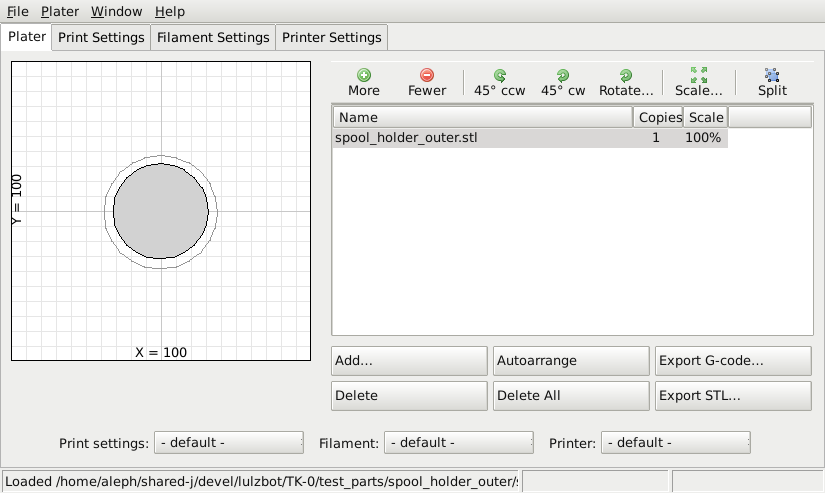
\includegraphics[keepaspectratio=true,angle=0,height=0.4\textheight,width=1.0\textwidth]{slic3r.png}
\caption{Slic3r application, STL to Gcode generator}
\label{fig:slic3r}
\end{figure}

Slic3r uses commonly used \texttt{.STL} files to create \texttt{.gcode} files. Gcode files contain instructions for the 3D printer on where, when, and how fast to make movements. However, Gcode programming is not very suitable for CAD and 3D design. This is where Slic3r and the \texttt{.STL} file comes into use. The \texttt{.STL} file is a 3D model file that can be exported by all common CAD and 3D modeling software. The Slic3r software then slices the \texttt{.STL} 3D model into layers and print paths to create a 3D printable \texttt{.gcode} file.

To launch Slic3r navigate to the \texttt{Slic3r} directory and launch the \texttt{slic3r.pl} file. On GNU/Linux operating systems you may need to set the \texttt{slic3r.pl} file as executable. On other operating systems it may be called \texttt{slic3r.exe}.

\index{download}
Slic3r includes very simple settings that allow you to easily refine prints. You can create multiple configurations for changing printer setups including nozzle sizes and desired print resolution. For ease of use we have pre-defined Slic3r configurations available in the Support/Downloads section at \texttt{www.LulzBot.com}. Download the configurations to your \texttt{Slic3r} directory.

\index{configuration}
\subsection{Loading Configurations}
To load configurations press the \texttt{Load Config...} button. In the file browser that opens, locate the downloaded configuration files. Select the configuration file that matches the nozzle size currently installed on the printer (0.5mm nozzle is installed by default). Press \texttt{Open} and the pre-defined configuration will load into Slic3r. You can also save custom configurations for yourself by pressing the \texttt{Export Config...} button. A file browser will open that allows you to define a name and save your custom configuration. 

\index{STL}
\index{plater}
\subsection{Loading STL files}
To load an \texttt{.STL} 3D model file into Slic3r, activate the Plater tab and click the \texttt{Add...} button. In the file browser navigate to the \texttt{.STL} you wish to load and click \texttt{Open}. The silhouette of the model will appear in the Plater diagram. To print more than one copy of the model at a time select the model name from the list and click the \texttt{More} button. With each press of the \texttt{More} button an additional copy of the model will be added to Plater. To remove a copy of the model select the model name again and click \texttt{Less}. To completely remove the model from Plater select the model name and click \texttt{Delete}.

\index{gcode}
\subsection{Export Gcode files}
Once you have finished setting your part(s) in Plater you can generate the Gcode by clicking \texttt{Export G-Code...}. In the file browser navigate to where you would like to save the \texttt{.gcode} file and list a name to save the file as. Click \texttt{Save} and Slic3r will begin generating the \texttt{.gcode} file. When Slicer is finished you will receive a prompt. If you have created a plate with multiple model designs you can also use the \texttt{Export STL...} function to save an \texttt{.STL} file for quickly reproducing the same plate of models.
\end{comment}

\section{Printrun}
%%% XXX shouldn't have to do it this way.
%%% HOWTO get page number from section? Ala  sec:Printrun
\label{Printrun}
\index{extruder}
\index{extrusion}
\index{temperature}
\index{gcode}
\index{SD card}
\index{Printrun}
Website: \texttt{http://www.github.com/kliment/Printrun}

The host software, Printrun, is used to start up and control your 3D printer 
(Fig. \ref{fig:printrun}, page \pageref{fig:printrun}).
\begin{figure}[hbt]
\centering
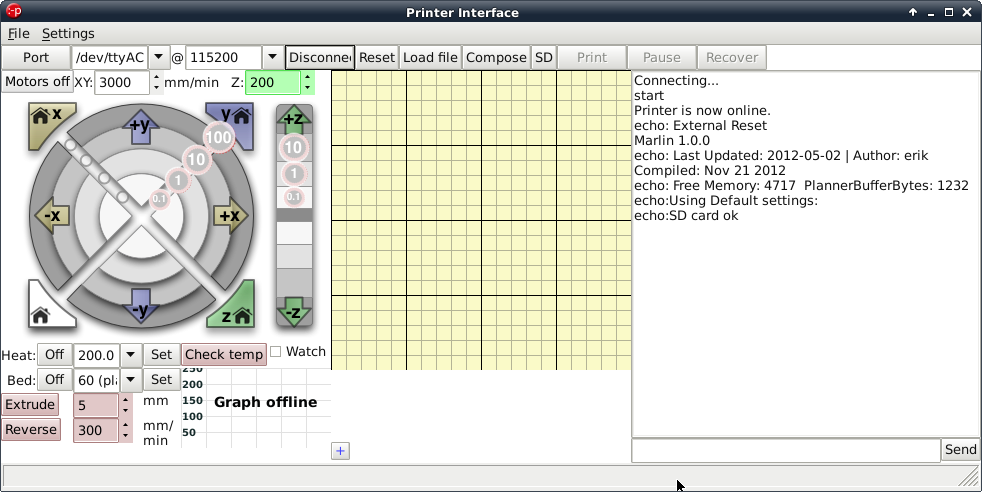
\includegraphics[keepaspectratio=true,angle=0,height=0.4\textheight,width=1.0\textwidth]{printrun.png}
\caption{Printrun application for 3D printer control}
\label{fig:printrun}
\end{figure}
The host controls include: setting the extruder and print surface temperatures, manual control of each axis, and manual extrusion. The host is also where you will push print files (\texttt{.gcode}) to the 3D printer or load print files from the SD card for printing out model designs.

\index{pronterface}
\index{GNU/Linux}
To launch Printrun, navigate to the \texttt{Printrun} directory and launch the \texttt{pronterface.py} file. On GNU/Linux operating systems you may need to set the \texttt{pronterface.py} file as executable. Depending on your environment you may need to launch the program by using the full command: \texttt{python pronterface.py}. On other operating systems the file may be called \texttt{pronterface.exe}.

\subsection{Connecting the Printer}
\index{connecting}
\index{Printrun}
\index{USB cable}
\index{port}
\index{baud rate}
\glossary{Baud Rate}{Refers to the speed at which the host controller communicates with the 3d Printer electronics.}
To start up the printer, first you will need to connect to the printer with Printrun. Make sure you have connected the USB cable from your PC to the printer before launching Printrun. If not, close Printrun, connect the USB cable, and relaunch Printrun. In the top left \texttt{Port} pull down menu select the correct port for the printer (generally \texttt{/dev/ttyACM0}). On other operating systems the port may be named such as \texttt{COM1} or \texttt{tty.usbserial-USB-ID}. If you only have one printer connected there will only be one port available to select. Make sure the port baud rate is set to \texttt{115200} in the pull down menu to the right of the port selection. You can refresh the USB ports, by clicking the \texttt{Port} button.

Now, to connect to the printer click the \texttt{Connect} button. In the text output window you will see multiple return lines. If you see \texttt{Printer is now online} you have successfully connected to the printer. The printer control buttons on the left will also darken and become click-able after connecting. When you need to disconnect the printer simply press the \texttt{Disconnect} button.

\subsection{Printer Controls}
\index{Printrun}
\index{hot end}
All of the printer controls can be found on the left side of the Printrun interface
(Fig. \ref{fig:printrun_controls}, page \pageref{fig:printrun_controls}).
\begin{figure}[hbt]
\centering
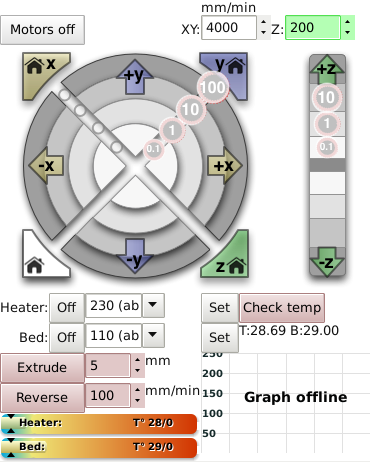
\includegraphics[keepaspectratio=true,angle=0,height=0.4\textheight,width=1.0\textwidth]{printrun_controls.png}
\caption{Printrun controls}
\label{fig:printrun_controls}
\end{figure}
To set the hot end and print surface temperature first click the \texttt{Monitor Printer} check box on. This will enable the printer temperature bars and graph. The hot end and print surface controls are labeled \texttt{Heater} and \texttt{Bed}. Select the temperature setting by using the pull down menu for pre-defined temperature settings. You can also set custom temperature settings by typing into the temperature box.

\index{temperature}
To turn on the hot end and/or printer surface click the respective \texttt{Set} button. The \texttt{Set} button will highlight orange when the temperature is set to on for that component. When the hot end or print surface is set to on you will see the temperature bar and graph display the set temperature and the current temperature. When both components have reached the correct temperature, the printer is ready for printing. Clicking the \texttt{Off} button will turn off that component and highlight the \texttt{Off} button blue.

\index{extrude}
\index{hot end}
Below the temperature controls are the manual extrusion controls. There you can manually extrude plastic through the hot end and retract the plastic filament from the hot end. The \texttt{Extrude} button will feed the amount of plastic, set to the right in mm, through the hot end. The rate at which the plastic is fed is set below the extrusion length (mm/min). The \texttt{Reverse} button will perform the opposite of \texttt{Extrude}, pulling the plastic filament back out of the hot end.

\index{manual controls}
\index{axes}
\index{X axis}
\index{Y axis}
\index{Z axis}
The large pattern of buttons above the temperature controls are the axes manual controls. These functions allows you to manually move each of the three axes of the printer. The circular pattern of four quadrants controls the X and Y axes. The top and bottom quadrants move the Y axis; the top in the positive direction (forward) and the bottom in the negative direction (back). The left and right quadrants move the X axis; the left in the negative direction (left) and the right in the positive direction (right).

Each quadrant is split into four sections that control the length of movement of 0.1mm, 1mm, 10mm, or 100mm. The innermost section moves the axis 0.1mm with each section outwards a larger movement with the outside section moving the axis 100mm.

The linear control bar to the right controls the Z axis. The Z axis is also separated into multiple movement lengths; 0.1mm, 1mm, and 10mm. The upper three buttons move the Z axis up and away from the printer surface; the three lower buttons move the Z axis closer to the print surface.

\index{home}
The four triangular buttons around the circular pattern are the axes home buttons. Each home button will move that axis in the negative direction until the end stop is activated. There is a home button for the X, Y, and Z axes. There is also a white home all button that homes all of the axes at once.

\index{motors}
The \texttt{Motors off} button will deactivate all motors allowing all of the axes to be moved by hand.

\index{end stops}
Caution: when homing, the axis will continue to move in the negative direction until the end stop switch is activated. If the printer is ever transported make sure the end stop switches are clear before resuming printing. If an axis has missed an end stop and is continuing to try to move in the negative direction, immediately turn the power switch to the off position. If a print file was running, after turning the power switch to off, pause the print by clicking the \texttt{Pause} button. Realign the end stop and try homing again.

\subsection{Loading Print Files}
\index{load files}
\index{gcode}
\index{Printrun}

To load a \texttt{.gcode} file into Printrun click the \texttt{Load file} button. Navigate to the \texttt{.gcode} file in the file browser and click \texttt{Open}. You will now see a 2D images of the first layer of your model design in the Gcode viewer
(Fig. \ref{fig:printrun_viewer}, page \pageref{fig:printrun_viewer}).
\begin{figure}[hbt]
\centering
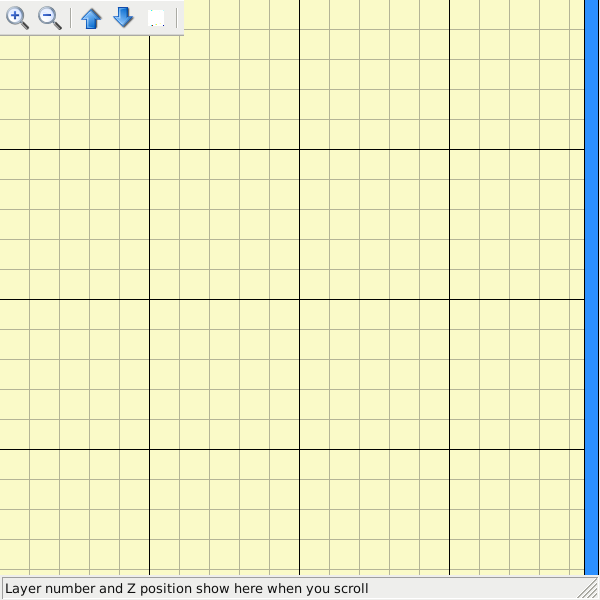
\includegraphics[keepaspectratio=true,angle=0,height=0.4\textheight,width=1.0\textwidth]{printrun_viewer.png}
\caption{Printrun viewer}
\label{fig:printrun_viewer}
\end{figure}
Click the Gcode viewer window to see a more detailed version of the sliced model. In the pop-up Gcode viewer you can zoom in using the mouse scroll wheel and flip through layers with the up and down arrow keys. To pan within the window left-click and drag to move around the work plane. The lines shown in the Gcode viewer represent the path the extrusion nozzle will follow to print the model.

For more information on using Printrun see the Printrun page in the Support/Downloads section at \texttt{https://www.lulzbot.com/?q=support}. Instructions for running a print can be found in the
%%% XXX Tag this
Starting the First Print section in this manual.

\section{CAD and 3D Modeling Software}
\index{CAD}
\index{software}
\index{STL}

Currently LulzBot is not distributing a CAD or 3D modeling software package. However, there are multiple free/libre software packages available. Other common non-free CAD and 3D modeling software are also capable of exporting the required \texttt{.STL} files.

On some CAD and 3D modeling software you will need to select millimeters as the output unit. If possible it is best to build your 3D design in metric units rather than imperial units. Slic3r requires .STL files sized in millimeters. If an .STL with inches as units is loaded into the Slic3r, the model will be scaled much smaller than expected. The software listed below outputs millimeters as the unit by default.

\subsection{FreeCAD}
\index{FreeCAD}
\index{GNU/Linux}
\index{Windows}
\index{Apple OS X}
Website: \texttt{http://free-cad.sourceforge.net}

Although still in development, FreeCAD is a great free/libre CAD application. Containing a full GUI for building CAD models, FreeCAD is capable of creating simple to complex designs. STL files can also easily be exported for use with 3D printing. FreeCAD is available for GNU/Linux, Windows, and Mac. The latest development version is recommended.

\subsection{OpenSCAD}
\index{OpenSCAD}
\index{GNU/Linux}
\index{Windows}
\index{Apple OS X}
Website: \texttt{http://openscad.org}

OpenSCAD is another free/libre CAD software; however, different than FreeCAD, it is script based. Rather than using a GUI to generate CAD designs, OpenSCAD CAD designs are created using script based renderings. Users with programming experience would find this very useful. Also, OpenSCAD uses a simple script language that is easy to learn for users with little or no programming experience.

\subsection{Blender}
\index{Blender}
\index{GNU/Linux}
\index{Windows}
\index{Apple OS X}
Website: \texttt{http://blender.org}

The most widely used Free/Libre 3D modeling software, Blender is well documented with tutorials available on the Blender.org website. Numerous video tutorials can be also found online.

